\documentclass[a4paper,12pt]{book}
% packages
\usepackage[utf8]{inputenc}
\usepackage[english]{babel}
\usepackage{fancyhdr}
\usepackage{bm}
\usepackage[a4paper]{geometry}
\geometry{margin=1in}
\usepackage{graphicx}
\graphicspath{{./images/}}
\usepackage[font=small,labelfont=bf]{caption}
\usepackage{subcaption}
\usepackage{fullpage}
\usepackage{setspace}
\usepackage{amsthm}
\usepackage{amsmath}
\usepackage{amssymb}
\usepackage{amsfonts}
\usepackage{enumitem}
\usepackage{mathtools}
\usepackage{booktabs}
\usepackage{commath}
\usepackage{multirow}
%\usepackage[newfloat]{minted}
\usepackage{csquotes}
\usepackage[hidelinks]{hyperref}
\usepackage[ruled,vlined]{algorithm2e}
\SetKwProg{Function}{Function}{:}{end}
\SetKwBlock{Main}{main()}{end}
\SetKwInOut{KwParam}{Parameters}
\usepackage{etoolbox}
\AtBeginEnvironment{algorithm}{\SetArgSty{textrm} \SetAlgoLined \DontPrintSemicolon \SetNoFillComment}
\usepackage[table,xcdraw]{xcolor}

\begin{document}
	
\begin{titlepage}
	
\frontmatter

\begin{center}
	% Upper part of the page
	
\includegraphics[scale=.10]{unipd.png}
	\\
	\vspace{1cm}
	\textsc{\LARGE University of Padova} \\
	\vspace{1cm}
	\textsc{\Large Information Engineering Department (DEI)} \\
	\vspace{1cm} 
	\textsc{\Large Master's Degree in Computer Engineering} \\ %\hspace{0.8cm}
	% Title
	\vspace{0.8cm}
	\Huge \doublespacing \bfseries \begin{spacing}{1}{Implementation of the ZI-Round heuristic for Mixed Integer Programming}\end{spacing}
	\hfill
	\Large \bfseries \begin{spacing}{1}{Master Thesis}\end{spacing}
	\hfill
	\vspace{0.5cm}
	% Author and supervisor
	\begin{flushleft} \large
		\emph{Supervisor:} \\
		Prof. Domenico Salvagnin
	\end{flushleft}
	\vfill
	\begin{flushright} \large
		\emph{Student:}\\
		Ivan Viviani (1206151)
	\end{flushright}
	\hfill
	\vfill
	% Bottom of the page
	{\small Academic Year 2019/2020} 
\end{center}
\end{titlepage}
	
\tableofcontents

\pagestyle{fancy}
\fancyhf{}
\fancyhead[RE,LO]{\rightmark}
\fancyfoot[CE,CO]{\thepage}
\renewcommand{\headrulewidth}{0pt}

\mainmatter

\chapter{Introduction}
%! Introduzione agli argomenti trattati nella tesi (ordine logico)

%! Organizzazione della tesi: presentazione in sequenza di quanto trattat nei singoli capitoli

\chapter{Mixed integer programming}
%! Small intro ??

\section{Mixed integer problems (MIPs)}
%! Definizione di MIP, tanti problemi reali (alcuni esempi) possono essere modellati con dei MIP -> bisogno di sviluppare algoritmi di risoluzione sempre più sofisticati -> MIP solvers (CPLEX, SCIP, Gurobi)

\section{MIP solvers}
%! MIP solvers: intro, test-bed selection, performance variability, branching and cutting planes (briefly, cite), presolving, primal heuristics (briefly, algorithmic/pragmatic), cite the others

\chapter{Primal heuristics}
%! Primal heuristics (Starting vs improvement in CPLEX) + general comments

\section{Start heuristics}
%! Aim of start heuristics

\subsection{Diving heuristics}
%! General description + cite examples (non sono il focus di questa tesi)

\subsection{Rounding heuristics}
%! Structure of rounding heuristics
%! Rounding strategies
%! Simple Rounding (brief) → Mention ZI-Round (extension introduced by Wallace)
%! Rounding
%! Shifting

\section{Improvement heuristics}
%! General description + brief examples

\chapter{ZI-Round MIP rounding heuristic} \label{ch:ziround}

ZI-round is a MIP rounding heuristic introduced by C. Wallace \cite{wallace2010} as an extension of the Simple Rounding heuristic, which was introduced in the non-commercial solver SCIP \cite{scip}.
From a primal feasible solution of the MIP continuous relaxation, both heuristics aim at rounding all the fractional integer variables, in order to obtain a feasible solution of the MIP. Simple Rounding is a pure integer rounding heuristic because it only rounds fractional integer variables, while ZI-Round also takes other factors into account, such as the singletons of the constraints, where a singleton is defined as a continuous variable that appears in only one constraint. \par

\section{Simple Rounding}
As its name suggests, Simple Rounding is the most straightforward approach: it scans the integer variables once and only rounds those that can be trivially rounded, keeping all the constraints satisfied without affecting other factors such as the constraint slacks and singletons.
Recall that a variable can be trivially rounded up or down only if any up-shift or down-shift within its bounds keeps all the constraints satisfied. \par

\subsection{Trivial roundability}
Consider a "less than" constraint in which the fractional integer variable $x_j$ appears with a positive coefficient $a_{ij} > 0$. Since this constraint is satisfied as long as its row activity is less than its right hand side, $x_j$ could only be rounded down, causing the row activity to decrease without affecting the constraint satisfiability. For the same constraint, if the variable $x_j$ appears with a negative coefficient $a_{ij} < 0$ instead, $x_j$ could only be rounded up, with the same outcome.
Now consider a "greater than" constraint in which the fractional integer variable $x_j$ appears with a negative coefficient $a_{ij} < 0$. Since this constraint is satisfied as long as its row activity is greater than its right hand side, $x_j$ could only be rounded down, causing the row activity to increase without affecting the constraint satisfiability. For the same constraint, if the variable $x_j$ appears with a positive coefficient $a_{ij} > 0$, $x_j$ could only be rounded up, with the same outcome.
Finally, consider an equality constraint in which the fractional integer variable $x_j$ appears. Since this constraint is satisfied as long as its row activity is equal to its right hand side, $x_j$ cannot be rounded in either direction without affecting other factors. \par

The previous examples describe the concept of trivial roundability for a fractional integer variable $x_j$ in a single constraint. But in order for a variable to be trivially roundable in a given direction, it must be roundable in all the constraints that comprise it, without affecting factors other than the variable itself. 
Note that it suffices that a variable appears in an equality constraint for it not to be trivially roundable in either direction, i.e. Simple Rounding cannot round variables that appear in at least one equality constraint.
A formal characterization of trivial roundability for a variable $x_j$ in the case of rounding up follows.
A variable $x_j$ can be trivially rounded up if and only if all the following conditions apply:
\begin{itemize}
	\item In all the "less than" constraints containing $x_j$, the variable appears with a negative coefficient $a_{ij} < 0$;
	\item In all the "greater than" constraints containing $x_j$, the variable appears with a positive coefficient $a_{ij} > 0$;
	\item All the equality constraints do not contain $x_j$.
\end{itemize}
A variable $x_j$ can be trivially rounded down if and only if all the following conditions apply:
\begin{itemize}
	\item In all the "less than" constraints containing $x_j$, the variable appears with a positive coefficient $a_{ij} > 0$;
	\item In all the "greater than" constraints containing $x_j$, the variable appears with a negative coefficient $a_{ij} < 0$;
	\item All the equality constraints do not contain $x_j$.
\end{itemize}
\par

\subsection{Towards ZI-Round}
The simplicity of Simple Rounding comes from its adherence to trivial roundability, which allows it to round variables without worrying about any other factors. As noted previously, this simplicity comes at the cost of effectiveness, since equality constraints make all the contained variables un-roundable. This major weakness of Simple Rounding can be overcome by taking other factors into account, as done by C. Wallace \cite{wallace2010} in the case of the ZI-Round heuristic. Also note that since a variable is or is not trivially roundable independently of other variables, and each trivial rounding causes the row activity of the constraints to decrease in the case of "less than" constraints and to increase in the case of "greater than" constraints, Simple Rounding only needs to scan the variables once.

\section{ZI-Round}
The ZI-Round heuristic greatly extends Simple Rounding by allowing non-trivial roundings to be made and cleverly using the singletons of each constraint (if any) as an additional slack. Non-trivial roundings are those in directions that do not ensure constraint satisfiability, i.e. some constraints could be violated due to the rounding. The use of singletons is essential for equality constraints, since it gives them a slack to rely on for rounding their contained variables. \par

An optional extension that can be easily implemented in ZI-Round is to allow the unit shifting of non-fractional integer variables to improve the objective value, while still maintaining non-fractionality. This extension can be seen as a sort of local search heuristic \cite{linker1973} or intensification strategy, analogous to $k$-OPT improvement for TSPs when $k = 1$, but different since imrovements are made before an integral solution is found \cite{wallace2010}. \par

\subsection{Main idea}
In the context of ZI-Round, the attempt to round all the fractional integer variables of the solution is carried out as an optimization problem where the objective function to minimize to zero is the solution fractionality, only relative to the integer variables of the original MIP (binary variables included). The fractionality of a single variable $x_j$ can be expressed as:
\begin{equation}
	f(x_j) = \text{min}\{x_j - \lfloor x_j \rfloor, \lceil x_j \rceil - x_j\}
\end{equation}
The fractionality of the solution, only relative to integer variables, is then given by:
\begin{equation}\label{eq:zi}
	f(x) = \sum_{j \in I \cup B}f(x_j)
\end{equation}
In accordance with the original work by C. Wallace \cite{wallace2010} and the name of the heuristic, in the rest of this thesis the solution fractionality is referred to as $ZI(x)$. \par 

While Simple Rounding scans the variables only once, since each variable can be trivially roundable independently of the others, ZI-Round needs to scan them multiple times: non-trivial roundings, and unit shiftings if the improvement extension is implemented, can change the row activities in both directions, causing the constraint (and singleton) slacks to possibly influence the roundability of other variables. Programmatically, this translates to having an outer loop that allows to perform multiple rounds and an inner loop that scans the integer variables, representing a single round. The pseudocode of the ZI-Round heuristic is presented in Algorithm~\ref{alg:ziround}. \par 

\SetKwRepeat{Do}{do}{while}
\begin{algorithm}[htp]
	\KwIn{$x$: primal feasible solution of continuous relaxation.}
	
	\Function{\upshape \texttt{ziround}}{
		\BlankLine
		$\Delta^{up}$ $\gets$ $\star$ maximum variable up-shifts $\star$ \;
		$\Delta^{down}$ $\gets$ $\star$ maximum variable down-shifts $\star$ \;
		$CS$ $\gets$ $\star$ constraint slacks $\star$ \;
		$SS$ $\gets$ $\star$ singleton slacks $\star$ \;
		$c$ $\gets$ $\star$ objective function coefficients $\star$ \;
		$c^Tx$ $\gets$ $\star$ objective value $\star$ \;
		$f(x_j)$ $\gets$ $\star$ fractionality of variable $x_j$ $\forall j$ $\star$ \;
		$ZI(x)$ $\gets$ $\star$ solution fractionality ($= \sum_{j \in I \cup B}f(x_j)$) $\star$ \;
		\BlankLine
		\Do{$\star$ variable roundings found $\star$}{
			\BlankLine
			\ForEach{$\star$ integer/binary variable $x_j$ $\star$}{
				\BlankLine
				\uIf{$\star$ $x_j$ non-fractional $\star$} {
					\BlankLine
					$\star$ compute maximum shifts of $x_j$ (threshold $\varepsilon = 1$) $\star$ \;
					\BlankLine
					\If{$(c_j \geq 0 \wedge \Delta_{j}^{down} = 1) \vee (c_j \leq 0 \wedge \Delta_{j}^{up} = 1)$}{
						\BlankLine
						$\star$ round (shift) $x_j$ to improve $c^Tx$ $\star$ \;
						$\star$ update slacks $CS$ and $SS$ $\star$ \;
						$\star$ update $c^Tx$ $\star$ \;
						\BlankLine
					}
					\BlankLine
				}
				\ElseIf{$\star$ $x_j$ fractional $\star$}{
					\BlankLine
					$\star$ compute maximum shifts of $x_j$ (threshold $\varepsilon = 10^{-5}$) $\star$ \;
					\BlankLine
					\uIf{$\star$ both shifts improve $ZI(x)$ of the same amount $\star$}{
						\BlankLine
						$\star$ round $x_j$ to improve $c^Tx$ $\star$ \;
						$\star$ update slacks $CS$ and $SS$ $\star$ \;
						$\star$ update $c^Tx$ $\star$ \;
						\BlankLine
					}
					\uElseIf{$\star$ rounding $x_j$ up improves $ZI(x)$ more $\star$}{
						\BlankLine
						$x_j$ $\gets$ $x_j + \Delta_{j}^{up}$ \;
						$\star$ update slacks $CS$ and $SS$ $\star$ \;
						$\star$ update $c^Tx$ $\star$ \;
						\BlankLine
					}
					\ElseIf{$\star$ rounding $x_j$ down improves $ZI(x)$ more $\star$}{
						\BlankLine
						$x_j$ $\gets$ $x_j - \Delta_{j}^{down}$ \;
						$\star$ update slacks $CS$ and $SS$ $\star$ \;
						$\star$ update $c^Tx$ $\star$ \;
						\BlankLine
					}
				}
			}
		}
	}
	\caption{ZI-Round.}
	\label{alg:ziround}
\end{algorithm}

\subsection{Data structures}
Non-trivial roundings could violate some constraints, therefore we need to determine how much each variable can be shifted in either direction towards its nearest integers, without violating any constraint. This information is denoted by the two arrays $\Delta^{up}, \Delta^{down}$ with index $j$ over the variables of the MIP. So $x_j$ can be shifted to either $x_j + \Delta_{j}^{up}$ or $x_j - \Delta_{j}^{down}$. \par

Whenever a variable is non-trivially rounded, the slacks of the constraints in which it is involved change and affect the possible shifts of other variables. So we need to keep track of the current values of the constraint slacks, denoted by the array $CS$ with index $i$ over the constraints of the MIP.
ZI-Round also accounts for the singletons of each constraint, which generate a further constribution to the overall slack, referred to as singletons slack and denoted by the array $SS$ with index $i$ over the constraints of the MIP. \par 

\subsection{Singletons slack}
The singleton slack of a constraint is defined as the contribution to the row activity given by the singletons. It can be seen as a single variable comprising the contributions of the singletons. 
Since the singletons are continuous variables that appear in only one constraint, they can be shifted freely without affecting other constraints, thus their contribution to the row activity can be manipulated in order to keep the constraint satisfied while rounding fractional integer variables. For example, consider the constraint $x_1 + x_2 + x_3 = 10$ where $x_1 = 3$, $x_2 = 4.5$, $x_3 = 2.5$, $x_2$ is the fractional integer variable that has to be rounded and $x_3$ is a singleton of the constraint. The only way to round $x_2$ is to use the available row activity contribution of $2.5$ given by $x_3$ to compensate for the shift: e.g. if $x_2$ is rounded up to $5$ then $x_3$ needs to be shifted down to $2$, and the constraint remains satisfied. \par 

\subsection{Maximum variable shifts}
Before any rounding can be performed, we need to determine the maximum up-shifts and down-shifts of the integer variables. To maintain primal feasibility, a variable shift must keep all the slacks of "less than" constraints non-negative, all the slacks of "greater than" constraints non-positive, and all the slacks of equality constraints equal to zero, intended as constraint slacks. \par

Consider an integer variable $x_j$ for which we want to determine $\Delta_{j}^{up}$ and $\Delta_{j}^{down}$.
For a "less than" constraint of index $i$ where $x_j$ has a positive coefficient $a_{ij} > 0$, the maximum up-shift of $x_j$ that can be compensated by the overall slack is given by $(CS_i + \Delta_{max}^{down}(SS_i)) / a_{ij}$, where $\Delta_{max}^{down}(SS_i))$ is the maximum down-shift of the singletons slack $SS_i$. Note that for $a_{ij} < 0$ the variable $x_j$ is trivially up-roundable in the constraint.
For a "less than" constraint of index $i$ where $x_j$ has a negative coefficient $a_{ij} < 0$, the maximum down-shift of $x_j$ that can be compensated by the overall slack is given by the same expression with a minus sign to keep the final value unsigned, i.e. $-(CS_i + \Delta_{max}^{down}(SS_i)) / a_{ij}$. Note that for $a_{ij} > 0$ the variable $x_j$ is trivially down-roundable in the constraint. In both the previous cases we consider the maximum down-shift of $SS_i$ because for "less than" constraints it is the one that increases the absolute value of the numerator, thus the final value, since $CS_i \geq 0$. \par 
For a "greater than" constraint of index $i$ where $x_j$ has a negative coefficient $a_{ij} < 0$, the maximum up-shift of $x_j$ that can be compensated by the overall slack is given by $(CS_i - \Delta_{max}^{up}(SS_i)) / a_{ij}$, where $\Delta_{max}^{up}(SS_i))$ is the maximum up-shift of the singletons slack $SS_i$. Note that for $a_{ij} > 0$ the variable $x_j$ is trivially up-roundable in the constraint.
For a "greater than" constraint  of index $i$ where $x_j$ has a positive coefficient $a_{ij} > 0$, the maximum down-shift of $x_j$ that can be compensated by the overall slack is given by the same expression with a minus sign to keep the final value unsigned, i.e. $-(CS_i - \Delta_{max}^{up}(SS_i)) / a_{ij}$. Note that for $a_{ij} < 0$ the variable $x_j$ is trivially down-roundable in the constraint. In both the previous cases we consider the maximum up-shift of $SS_i$ because for "greater than" constraints it is the one that increases the absolute value of the numerator, thus the final value, since $CS_i \leq 0$. \par
Equality constraints can exclusively rely on their singletons slack, which unlike the constraint slack can be positive or negative. So an equality constraint can be viewed as a "less than" constraint when its singletons slack is positive and as a "greater than" constraint when its singletons slack is negative. For an equality constraint of index $i$ where $x_j$ has a positive coefficient $a_{ij} > 0$, the maximum up-shift of $x_j$ that can be compensated by the singletons slack is given by $\Delta_{max}^{down}(SS_i) / a_{ij}$, while the maximum down-shift is given by $\Delta_{max}^{up}(SS_i) / a_{ij}$. For an equality constraint of index $i$ where $x_j$ has a negative coefficient $a_{ij} < 0$, the maximum up-shift of $x_j$ that can be compensated by the singletons slack is given by $-\Delta_{max}^{up}(SS_i) / a_{ij}$, while the maximum down-shift is given by $-\Delta_{max}^{down}(SS_i) / a_{ij}$. \par 

All the considerations made so far hold for a single constraint, but in order to keep all the constraints satisfied we need to find the minimum over all the constraints of such maximum quantities. The idea is that each constraint gives two candidates for $\Delta_{j}^{up}$ and $\Delta_{j}^{down}$, respectively. Then the final maximum shifts of $x_j$ are determined as the minimum candidate for each rounding direction. 
Note that the variables also have to stay within their lower and upper bounds, so two additional candidates are given by the quantities $x_j - lb_j$ for $\Delta_{j}^{down}$ and $ub_j - x_j$ for $\Delta_{j}^{up}$, where $lb_j$ and $ub_j$ denote the variable bounds.
A more formal characterization of the maximum up-shift and down-shift of a variable $x_j$ follows. \par

For "less than" constraints, a variable $x_j$ cannot be shifted up more than
\begin{equation}
	\Delta_{j,\leq}^{up} = \min_{i,\leq}\left\{\dfrac{(CS_i + \Delta_{max}^{down}(SS_i))}{a_{ij}} : a_{ij} > 0\right\}
\end{equation}
and it cannot be shifted down more than
\begin{equation}
	\Delta_{j,\leq}^{down} = \min_{i,\leq}\left\{\dfrac{-(CS_i + \Delta_{max}^{down}(SS_i))}{a_{ij}} : a_{ij} < 0\right\}
\end{equation}

For "greater than" constraints, a variable $x_j$ cannot be shifted up more than
\begin{equation}
	\Delta_{j,\geq}^{up} = \min_{i,\geq}\left\{\dfrac{(CS_i - \Delta_{max}^{up}(SS_i))}{a_{ij}} : a_{ij} < 0\right\}
\end{equation}
and it cannot shifted down more than
\begin{equation}
	\Delta_{j,\geq}^{down} = \min_{i,\geq}\left\{\dfrac{-(CS_i - \Delta_{max}^{up}(SS_i))}{a_{ij}} : a_{ij} > 0\right\}
\end{equation}

For equality constraints, a variable $x_j$ cannot be shifted up more than
\begin{equation}
	\Delta_{j,=}^{up} = \min \left\{ \min_{i,=}\left\{\dfrac{\Delta_{max}^{down}(SS_i)}{a_{ij}} : a_{ij} > 0\right\} , \min_{i,=}\left\{\dfrac{-\Delta_{max}^{up}(SS_i)}{a_{ij}} : a_{ij} < 0 \right\} \right\}
\end{equation}
and it cannot be shifted down more than
\begin{equation}
	\Delta_{j,=}^{down} = \min \left\{ \min_{i,=}\left\{\dfrac{\Delta_{max}^{up}(SS_i)}{a_{ij}} : a_{ij} > 0\right\} , \min_{i,=}\left\{\dfrac{-\Delta_{max}^{down}(SS_i)}{a_{ij}} : a_{ij} < 0 \right\} \right\}
\end{equation}

Grouping the three types of constraints together and considering also the additional candidates given by the variable bounds yields the final values of the maximum shifts of $x_j$ that maintain primal feasibility:
\begin{equation}
	\Delta_{j}^{up} = \text{min} \{\Delta_{j,\leq}^{up} \,,\, \Delta_{j,\geq}^{up} \,,\, \Delta_{j,=}^{up} \,,\, ub_j - x_j\}
\end{equation}
\begin{equation}
	\Delta_{j}^{down} = \text{min} \{\Delta_{j,\leq}^{down} \,,\, \Delta_{j,\geq}^{down} \,,\, \Delta_{j,=}^{down} \,,\, x_j - lb_j\}
\end{equation}

One detail that speeds up the ZI-Round heuristic, as recommended by C. Wallace \cite{wallace2010}, is to stop calculating $\Delta_{j}^{up}$ and $\Delta_{j}^{down}$ once they both fall below a pre-defined small positive threshold, denoted by $\varepsilon$. In practice we use the same value chosen by C. Wallace, i.e. $\varepsilon = 10^{-5}$. If the ZI-Round extension that shifts non-fractional integer variables is implemented, as done in this thesis, for determining the possible shifts in that case it suffices to set the threshold $\varepsilon = 1$, because $x_j$ must be shifted by $1$ to maintain the current solution fractionality $ZI(x)$. \par

\subsection{Objective improving shifts}
As presented in the inner loop of Algorithm~\ref{alg:ziround}, if the current variable $x_j$ is non-fractional then the improvement extension is applied, whereas if $x_j$ is fractional then it enters the core of the ZI-Round heuristic. As initially mentioned, ZI-Round aims at minimizing the solution fractionality $ZI(x)$ expressed by Equation~\ref{eq:zi}, therefore $x_j$ should be rounded in the direction that improves $ZI(x)$, with ties resolved in favor of the direction that improves the objective value $c^Tx$. \par
The pseudocode of the function that, given both the maximum shifts of a variable $x_j$, shifts it in the direction that improves $c^Tx$ is presented in Algorithm~\ref{alg:roundxjbestobj}. Particular care must be taken when non-fractional integer variables have to be shifted by this function: it is important to ensure that $ZI(x)$ is maintained by checking that the shift applied has a value of $1$. \par

\begin{algorithm}[ht]
	\KwIn{$j$: variable index; $\Delta_{j}^{up}$: maximum variable up-shift; $\Delta_{j}^{down}$: maximum variable down-shift.}

	\Function{\upshape \texttt{round\_xj\_bestobj}}{
		\BlankLine
		$CS$ $\gets$ $\star$ constraint slacks $\star$ \;
		$SS$ $\gets$ $\star$ singleton slacks $\star$ \;
		$c$ $\gets$ $\star$ objective function coefficients $\star$ \;
		$c^Tx$ $\gets$ $\star$ objective value $\star$ \; 
		\BlankLine
		\uIf{$\star$ rounding $x_j$ up improves $c^Tx$ more $\star$}{
			\BlankLine
			$x_j$ $\gets$ $x_j + \Delta_{j}^{up}$ \;
			$\star$ update slacks $CS$ and $SS$ $\star$ \;
			$\star$ update $c^Tx$ $\star$ \;
			\BlankLine
		}
		\uElseIf{$\star$ rounding $x_j$ down improves $c^Tx$ more $\star$}{
			\BlankLine
			$x_j$ $\gets$ $x_j - \Delta_{j}^{down}$ \;
			$\star$ update slacks $CS$ and $SS$ $\star$ \;
			$\star$ update $c^Tx$ $\star$ \;
			\BlankLine
		}
		\ElseIf{$\star$ both shifts improve $c^Tx$ of the same amount ($0$ included) $\star$}{
			\BlankLine
			$\star$ round $x_j$ arbitrarily $\star$ \;
			$\star$ update slacks $CS$ and $SS$ $\star$ \;
			$\star$ update $c^Tx$ $\star$ \;
			\BlankLine
		}
	}
	\caption{Round $x_j$ to improve objective.}
	\label{alg:roundxjbestobj}
\end{algorithm}

\subsection{Slacks update}
After any rounding has been made, we need to update the constraint slacks $CS$ and possibly the singletons slacks $SS$. The pseudocode of the function that, given the signed shift that was used to round a variable $x_j$, computes the corresponding slack shift for each constraint of index $i$ and distributes it on the constraint slack $CS_i$ and/or the singletons slack $SS_i$ (if any) is presented in Algorithm~\ref{alg:updateslacks}. \par
The function scans the constraints containing the integer variable $x_j$ and updates the slacks. For each constraint of index $i$ it first computes the signed overall slack shift corresponding to the signed variable shift $\Delta_{j}$, given by:
\begin{equation}
	\Delta_{i}^{slack} = a_{ij} \Delta_{j}
\end{equation}
where $a_{ij}$ is the coefficient of $x_j$ in the constraint. Then as much of the overall slack shift as possible is distributed on the constraint slack $CS_i$. If the constraint has any singletons, $CS_i$ could not be able to compensate for all of $\Delta_{i}^{slack}$, so in this case the remaining slack shift $\Delta_{i}^{SS}$ has to be distributed on the singletons slack $SS_i$, thus among the singletons of the constraint. \par

Note that since the singletons of the constraint are actual variables of the MIP, an update of the singletons requires to update the current objective value $c^Tx$. Also, observe that the slacks are updated only after a successful rounding or shifting, therefore $\Delta_{i}^{slack}$ can always be distributed correctly. \par

\begin{algorithm}[ht]
	\KwIn{$j$: index of the rounded variable; $\Delta_{j}$: signed variable shift.}
	
	\Function{\upshape \texttt{update\_slacks}}{
		\BlankLine
		$CS$ $\gets$ $\star$ constraint slacks $\star$ \;
		$SS$ $\gets$ $\star$ singleton slacks $\star$ \;
		\BlankLine
		\ForEach{$\star$ constraint containing $x_j$ $\star$}{
			\BlankLine
			$a_{ij}$ $\gets$ $\star$ coefficient of $x_j$ in $i^{th}$ constraint $\star$ \;
			$\Delta_{i}^{slack}$ $\gets$ $\star$ slack shift of the constraint ($= a_{ij} \, \Delta_{j}$) to be distributed $\star$ \;
			\BlankLine
			\uIf{$\star$ constraint sense $\leq$ or $\geq$ $\star$}{
				\BlankLine
				\uIf{$\star$ constraint has singletons $\star$} {
					\BlankLine
					$\star$ update constraint slack $CS_i$ to cover $\Delta_{i}^{slack}$ as much as possible $\star$ \;
					$\Delta_{i}^{SS}$ $\gets$ $\star$ remaining slack shift (covered by the singletons) $\star$ \;
					$SS_i$ $\gets$ $SS_i + \Delta_{i}^{SS}$ \;
					$\star$ update constraint singletons by distributing $\Delta_{i}^{SS}$ (if any) $\star$ \;
					$\star$ update $c^Tx$ if singletons were updated $\star$ \;
					\BlankLine
				}
				\Else{
					\BlankLine
					$\star$ update constraint slack $CS_i$ $\star$ \;
					\BlankLine
				}
				\BlankLine
			}
			\ElseIf{$\star$ constraint sense $=$ $\star$}{
				\BlankLine
				\If{$\star$ constraint has singletons $\star$}{
					\BlankLine
					$\Delta_{i}^{SS}$ $\gets$ $\Delta_{i}^{slack}$ \;
					$SS_i$ $\gets$ $SS_i + \Delta_{i}^{SS}$ \;
					$\star$ update constraint singletons by distributing $\Delta_{i}^{SS}$ $\star$ \;
					$\star$ update $c^Tx$ $\star$ \;
					\BlankLine
				}
			}
		}
	}
	\caption{Update slacks.}
	\label{alg:updateslacks}
\end{algorithm}

On a final note, the observations and experimental results of C. Wallace \cite{wallace2010} show that ZI-Round can round any variable that Simple Rounding can round, while maintaining similar overall running times, but ZI-Round can find more solutions.

\chapter{ZI-Round extensions}
In this thesis the implementation of ZI-Round that takes the singletons into account and employs the extension of improving the objective value by shifting non-fractional integer variables while rounding the fractional ones is referred to as the default version, i.e. the one described in Chapter~\ref{ch:ziround}. \par
In this chapter, some variations and extensions of the ZI-Round heuristic are presented, together with some example charts showing the behavior of the solution cost and fractionality as the inner loop iterations of ZI-Round progress. Note that only one feature at a time is changed from the default ZI-Round implementation: all the features of default ZI-Round are kept, except for the one changed by each extension.
Eventually, a new default version of ZI-Round is proposed. \par 
The charts presented are made by the author of this thesis using the Gnuplot graphing utility \cite{gnuplot}, called directly from the main program through a pipe. The data portrayed by the charts is obtained from the experiments conducted, which are described in detail in Chapter~\ref{ch:compresults}.

\section{Default ZI-Round}
The default version of ZI-Round shifts both fractional and non-fractional integer variables, the latter to improve the objective value.
The two phases of rounding and objective improvement are overlapped, causing the solution cost to vary unsteadily until all the fractional integer variables have been rounded. The rounding phase terminates when the solution fractionality reaches zero and from that point on the objective improvement phase continues until no more improvements are possible.
A visual example of such behavior is shown in Figure~\ref{fig:exzi-default} for the instance \texttt{fast0507}: the two phases coexist until the solution fractionality reaches zero, at which point only the objective value improvement occurs.
\begin{figure}[ht]
	\centering
	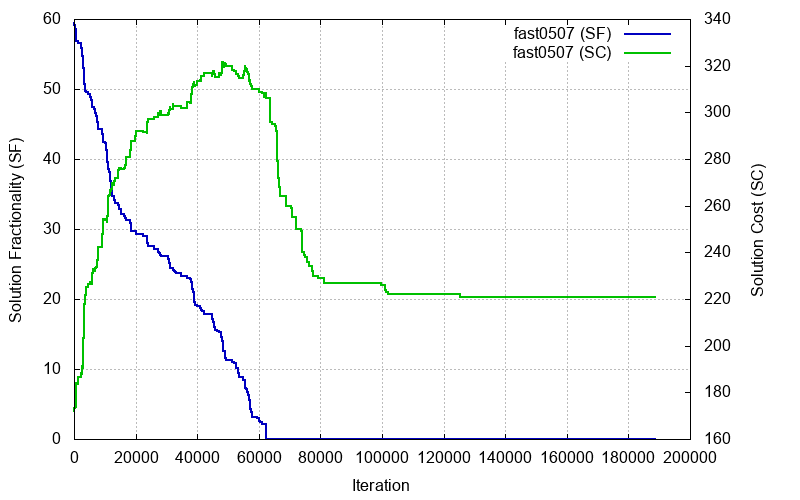
\includegraphics[width=\textwidth]{fast0507-default.png}
	\caption{ZI-Round execution for the instance \texttt{fast0507}: default.}
	\label{fig:exzi-default}
\end{figure}

\section{Sorted singletons}
A first simple extension follows from a possible improvement on the order in which the singletons of a given constraint are considered when distributing the singletons slack on them, with the aim of worsening the objective value as little as possible. \par 

In the default implementation of ZI-Round the singletons are considered in their natural order. The proposed improvement consists in sorting the singletons of each constraint in ascending order of their objective function coefficients, so that the first singleton variables to be updated are the ones that affect the objective value the least. \par

We recognize that this greedy approach does not ensure to always affect the objective value in a positive way, since the current possible singleton variations would need to be taken into account at each iteration, and those variations depend on the bounds of the singleton and its coefficient in the constraint. However, this simple extension is tested with the aim of showing whether and in what amount the order in which the singletons are considered influences the end results. The chosen reference instance does not have any singletons in its constraints, hence no example chart is available for this extension.

\section{No objective improvement}
Another extension of ZI-Round worth analyzing is the shift of non-fractional integer variables to improve the objective value as much as possible. Since this extension is part of the default version of ZI-Round, its complementary counterpart is considered, i.e. the absence of it. \par

The rationale behind this non-extension is the following. First, observe that the overall slack of a constraint can be viewed as its capacity to cover the possible shift of one of its variables, and a variable shift can either increase or decrease that capacity. Also, in a way, the constraints of a MIP should generally go against the objective function, otherwise the problem would be unbounded. It follows that shifting non-fractional integer variables to improve the objective value should contribute to the saturation of the shift coverage capacity of the constraints, which could not be able to allow all the fractional integer variables to be rounded. \par

This non-extension that avoids shifting non-fractional integer variables is tested with the aim of showing whether and in what amount the attempt to improve the objective value while rounding all the integer variables influences the end results, especially in terms of quality of the solutions found. \par

Without objective improvement, the rounding phase is free to operate and terminates as soon as the solution fractionality reaches zero, marking the end of the heuristic. A visual example of such behavior is shown in Figure~\ref{fig:exzi-noobjimprove} for the instance \texttt{fast0507}. Note that all the fractional integer variables are rounded after way less iterations with respect to the default version, which shows how the objective improvement phase interferes with the rounding phase, making the rounding process longer.
\begin{figure}[ht]
	\centering
	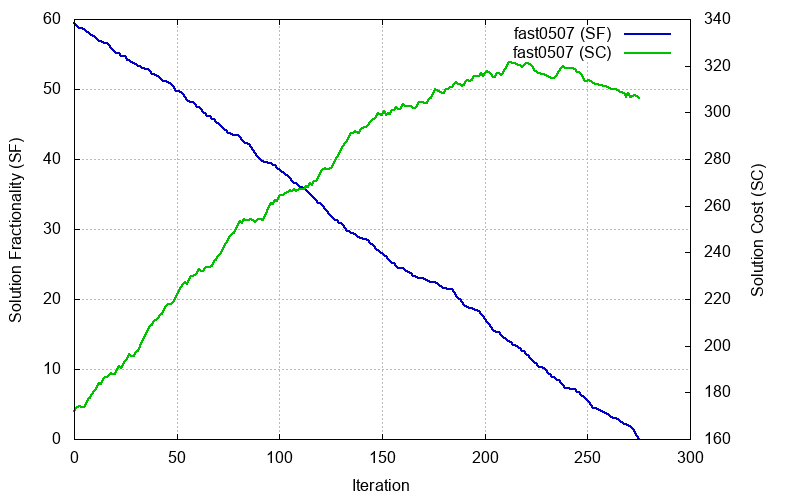
\includegraphics[width=\textwidth]{fast0507-noshiftnonfrac.png}
	\caption{ZI-Round execution for the instance \texttt{fast0507}: no objective improvement.}
	\label{fig:exzi-noobjimprove}
\end{figure}

\section{Objective improvement after zero fractionality}
The previous non-extension is a rather conservative approach that avoids any objective value imrovement from start to finish. \par 

A very reasonable extension that allows the fractional integer variables to fully rely on the slacks in order to be rounded and the objective value to be improved consists in starting to shift the non-fractional integer variables only after all the fractional ones have been rounded. In other words, this extension would follow the previous one until the fractionality of the solution reaches zero or no more fractional variables can be rounded, and then start improving the objective value by shifting all the integer variables, which would all be non-fractional at that point. \par

This two-phased extension that first concentrates on rounding all the fractional integer variables and only after no more fractional variables can be rounded proceeds to improve the objective value is tested with the aim of showing whether and in what amount separating the rounding phase and the objective improvement phase affects the end results. \par 

Since the two phases are separated, at first all the slacks are exclusively at the disposal of the rounding phase, which is prioritized. This separation is reflected in the behavior of the solution cost, which tends to increase while the fractionality approaches zero, at which point the objective improvement phase starts shifting the non-fractional integer variables, causing the objective value to decrease until no more improvements are possible. A visual example of such behavior is shown in Figure~\ref{fig:exzi-objimproveafter0frac} for the instance \texttt{fast0507}. The rounding phase is the same as in Figure~\ref{fig:exzi-noobjimprove}, with the solution fractionality of the instance reaching zero at iteration $275$, at which point the objective improvement phase starts operating until the end of the heuristic.
\begin{figure}[ht]
	\centering
	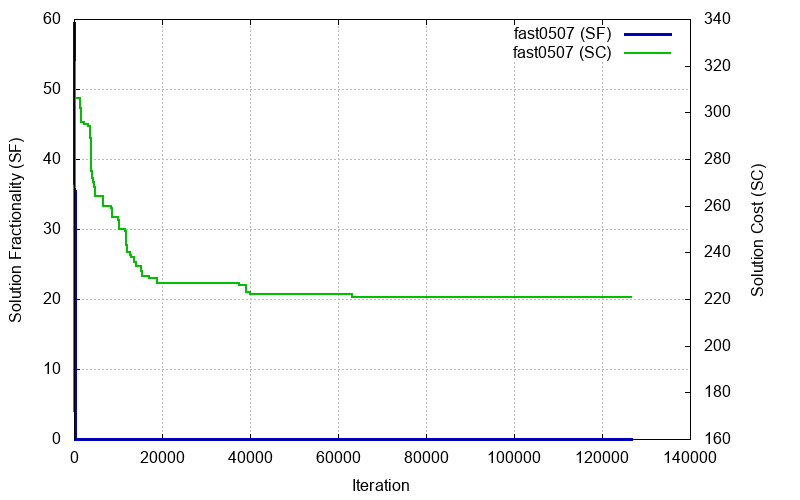
\includegraphics[width=\textwidth]{fast0507-shiftnfafter0frac.png}
	\caption{ZI-Round execution for the instance \texttt{fast0507}: objective improvement after zero fractionality.}
	\label{fig:exzi-objimproveafter0frac}
\end{figure}

\section{Worst-objective fractionality tie-breaks}
The final extension proposed follows from the observation that any attempt at improving the objective value generally goes against the capacity of the constraints to compensate for the shifts of the variables they contain. \par 

As reported in Algorithm~\ref{alg:ziround}, the default behavior of ZI-Round when fractionality tie-breaks occur during the rounding process of a fractional integer variable is to prefer the rounding direction that improves the objective value the most, or worsens it the least. This proposed extension, instead, in such cases would choose to round the variable in the direction that worsens the objective value the most, or improves it the least. This behavior would in fact favor the constraints, thus the possibility of rounding more fractional integer variables. \par

Note that the shifting of non-fractional integer variables of the default ZI-Round implementation is maintained. This mixed extension that favors both the objective function and the constraints is tested with the aim of showing whether and in what amount favoring the constraints when either direction can be chosen while rounding a fractional integer variable affects the end results. \par 

Since the direction that worsens the objective value is chosen whenever a tie on the fractionality improvement given by a possible shift occurs, in such cases more power is given to the rounding phase. On the other hand, the objective improvement phase still operates concurrently throughout the execution of the heuristic. A visual example of such behavior is shown in Figure~\ref{fig:exzi-fractieworstobj} for the instance \texttt{fast0507}: as expected, it is similar to the one obtained by the default version of ZI-Round, since the two phases still interfere with one another from the start.
\begin{figure}[ht]
	\centering
	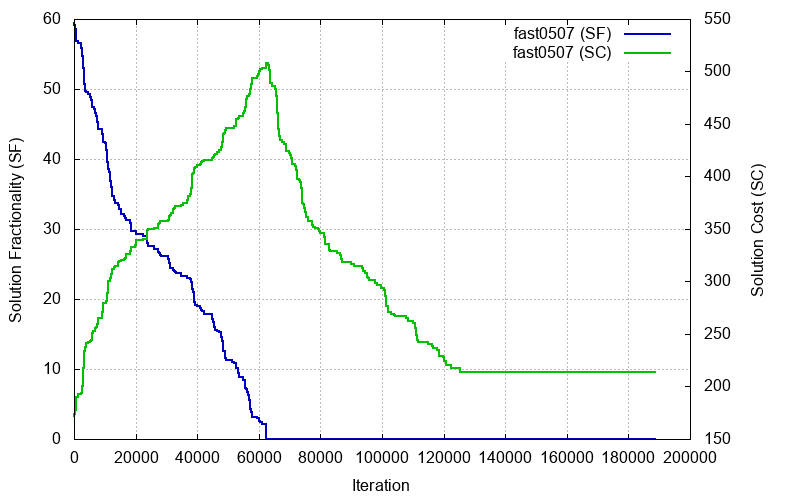
\includegraphics[width=\textwidth]{fast0507-fractieworstobj.png}
	\caption{ZI-Round execution for the instance \texttt{fast0507}: worst-objective fractionality tie-breaks.}
	\label{fig:exzi-fractieworstobj}
\end{figure}

\section{Proposed ZI-Round}
From the behaviors of the extensions observed and the experiments conducted, the following version of ZI-Round is proposed as the new default. The proposed ZI-Round heuristic employs the sorting of the singletons of each constraint, the worst-objective fractionality tie-breaks and the objective improvement after the fractionality reaches zero. The experimental results that support this choice are presented in Chapter~\ref{ch:compresults}. \par
The behavior of the solution cost and fractionality for the instance \texttt{fast0507} under the proposed version of ZI-Round is shown in Figure~\ref{fig:exzi-proposed}. Unlike in Figure~\ref{fig:exzi-objimproveafter0frac}, where the final objective value is $221$, in this case a solution with an objective value of $214$ is found.
\begin{figure}[ht]
	\centering
	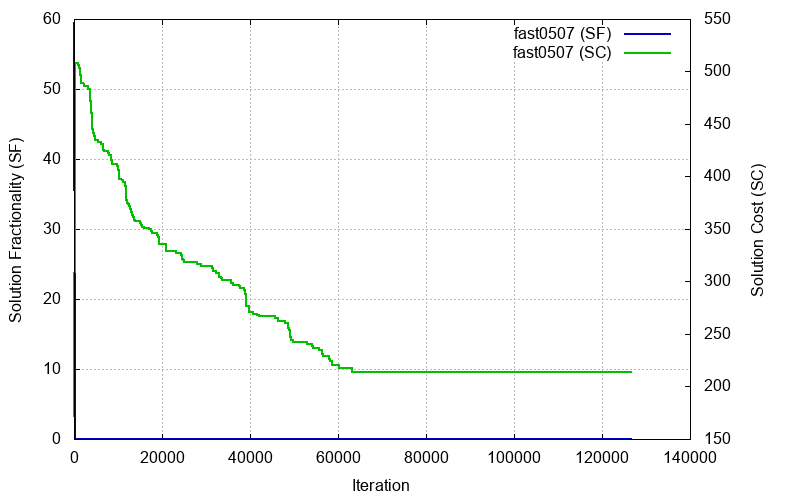
\includegraphics[width=\textwidth]{fast0507-proposed.png}
	\caption{ZI-Round execution for the instance \texttt{fast0507}: proposed.}
	\label{fig:exzi-proposed}
\end{figure}

\chapter{Computational results} \label{ch:compresults}
%! Scopo degli esperimenti: analizzare la performance di ZI-Round nelle sue varie estensioni/varianti in termini di numero di soluzioni intere trovate e tempo di esecuzione.
The performance of the ZI-Round heuristic is analyzed in the following experiments, in which one extension at a time is changed from the default version. The main measures of interest are the number or percentage of integer solutions found, the quality of those solutions and the execution time of ZI-Round. \par 

First, in Section~\ref{sec:preliminary-exp}, two preliminary experiments are carried out: the first one concerning the comparison between the results obtained by default ZI-Round and those reported by C. Wallace  for the successful instances in \cite{wallace2010}; the second one concerning the comparison between the results obtained by default ZI-Round and those obtained by the \textit{zirounding} heuristic implemented in the non-commercial solver SCIP, on the same test-bed used by C. Wallace. These experiments serve as confirmation of the reliability of the ZI-Round implementation made by the author of this thesis. \par

In Section~\ref{sec:expsetup}, the experimental setup used for the set of experiments on the different versions of ZI-Round is presented. In particular, it comprises the specification of the hardware and software tools used, the description of the test-beds used for the experiments, the specification of the single measures performed on the instances and the aggregate measures computed on the test-beds. Also, a second interesting set of experiments that exploit the shift of dimensional space seen in the presolving process of CPLEX is introduced. \par 

In Section~\ref{sec:expresults} the experimental results on the test-beds described are presented and discussed, together with some example charts showing the behavior of the ZI-Round versions tested in terms of solution fractionality and solution cost, on two reference instances. The charts presented are made by the author of this thesis using the Gnuplot graphing utility \cite{gnuplot}, called directly from the main program through a pipe. The data portrayed by the charts is obtained from the experiments conducted.

\section{Preliminary experiments} \label{sec:preliminary-exp}

\subsection{Comparison with ZI-Round v2}
After implementing the default version of the ZI-Round heuristic, referred to as ZI-Round version $2$ (v$2$) in the original work by C. Wallace \cite{wallace2010}, a quick replicability experiment is carried out to check whether the custom implementation of the author of this thesis finds similar resulting objective values to those found by the implementation of C. Wallace, for the successful instances reported in the article. In particular, the test-bed contains $18$ instances taken from the MIPLIB $2003$ problem set \cite{miplib2003}, from which one instance is removed since it has ranged constraints that make it incompatible with the custom implementation. \par
The results of the replicability experiment are reported in Table~\ref{tb:exp-prelim-1}: the implemented default version of ZI-Round found a solution for $13$ of the $17$ instances for which ZI-Round v$2$ found a solution.
\begin{table}[]
	\centering
	\begin{tabular}{@{}lrrr@{}}
	\toprule
	Instance   & ZI-Round(implemented) & ZI-Round(v2) & zirounding(SCIP) \\ \midrule
	cap6000    & -2446875              & -2446875     & -2442801         \\
	fast0507   & 221                   & 200          & 288              \\
	fixnet6    & 12170                 & 4536         & 4482             \\
	manna81    & -11868                & -13164       & -13150           \\
	markshare1 & 230                   & 230          & 418              \\
	markshare2 & 167                   & 674          & 375              \\
	mkc        & Failed                & -346      & Failed           \\
	modglob    & 20786787           & 20786788     & 20757201      \\
	nsrand-ipx & 754880                & 69600        & Failed           \\
	pp08a      & 15000                 & 14300        & 13940            \\
	pp08aCUTS  & 16630           & 16630      & 15147      \\
	qiu        & 1805           & 1805      & 1805      \\
	set1ch     & 110242              & 107692     & 106027           \\
	seymour    & 454                   & 450          & 615              \\
	sp97ar     & Failed                & 1094926720   & Failed           \\
	timtab1    & Failed                & 1719551      & Failed           \\
	timtab2    & Failed                & 2449798      & Failed           \\ \bottomrule
	\end{tabular}
	\caption{Objective values obtained by different implementations of the default ZI-Round heuristic.}
	\label{tb:exp-prelim-1}
\end{table}

The failure of the custom implementation in $4$ instances is further analyzed in a second experiment, by comparing the results with those obtained by the \textit{zirounding} heuristic integrated in the non-commercial solver SCIP version $7$.$0$.$0$ \cite{scip}, which could not be exctracted from the code of the version used in \cite{wallace2010}, leading to the implementation of ZI-Round v$2$. \par 

\subsection{Comparison with ZI-Round in SCIP}
To double check the reliability of the previous results, the test-bed is extended to the whole MIPLIB $2003$ problem set, which is the complete test-bed actually used by C. Wallace, from which the instances that are incompatible with ZI-Round are removed. The extended test-bed contains $59$ instances. The second preliminary experiment involves the comparison between default ZI-Round and \textit{zirounding}, to confirm the reliability of the implementation. \par 

The solver SCIP was downloaded with an academic license and set up to use only the \textit{zirounding} heuristic and stop the solving process at the root node of the decision tree. In particular, the following commands are issued:
\begin{enumerate}
	\item Disable all the heuristics: "\texttt{set heuristics emphasis off}"
	\item Enable only the \textit{zirounding} heuristic: "\texttt{set heuristics zirounding freq 1}"
	\item Set the node limit to $1$: "\texttt{set limits nodes 1}"
	\item Disable all cut separators: "\texttt{set separating emphasis off}"
\end{enumerate}
Once SCIP is set up, the command to optimize a given problem is the following: "\texttt{read filename.mps optimize}". The execution and success of \textit{zirounding} can be verified by issuing the command "\texttt{disp stats}" after the problem optimization. \par

The complete results of the second experiment are omitted since almost all the additional instances not reported in Table~\ref{tb:exp-prelim-1} are unsuccessful for both the implementations being compared.  \par 

The results obtained by SCIP present the same $4$ failures mentioned previously. With some slight differences, which could be due to the newer versions of the solvers being used or performance variability factors, the custom implementation of ZI-Round made by the author of this thesis can be deemed as a reliable instance of the heuristic to be tested in the following experiments.

\section{Experimental setup} \label{sec:expsetup}

\subsection{Hardware and software tools}
%! Strumenti: specifiche PC, software/tools usati
All the experiments are performed on a Dell XPS $15$ $7590$, with an exa-core $4.5$ GHz i$7$-$9750$H processor and $16$ GB of RAM, using the Windows $10$ Pro version $2004$ operating system. \par

%! Software/tools usati
The solver used for obtaining the solutions of the continuous relaxations is CPLEX version $12$.$10$.$0$ with an academic license \cite{cplex}. Its interactive optimizer is also used for presolving problems and writing them to \texttt{mps} files.
The Dirent C API \cite{dirent} is used for easily scanning the instance files to read in the test folder.
The Gnuplot \cite{gnuplot} graphing utility is used to programmatically create the charts presented in this thesis using pipes to pass commands and data points to it directly from the main program.
The R language \cite{rlang} is used to easily manage the test results and compute the aggregate measures of interest.

\subsection{Test-bed collection}

%! Testbed: MIPLIBS + tipologie di istanze rimosse + numero istanze testate
The test-bed used for the experiments comprises the instances from the MIPLIB $2003$ \cite{miplib2003}, MIPLIB $2010$ \cite{miplib2010} and MIPLIB $2017$ \cite{miplib2017} problem collections, from which the instances that are incompatible with ZI-Round are removed.
The removed instances include: instances that are infeasible or unbounded; instances that have ranged constraints; instances that have semi-integer or semi-continuous variables according to the terminology used by CPLEX; and instances for which CPLEX is unable to solve the continuous relaxation or exceeds a set time limit of $300$ seconds. To simplify the detection of removable instances, a single run in which only the continuous relaxations are solved is performed on the union of the three problem collections: the function \texttt{CPXgetstat} of the CPLEX C API is used to get the solution status and the instances that do not have the status \texttt{CPX\_STAT\_OPTIMAL} are removed from the test-bed. After this pre-processing run, the test-bed obtained contains $1102$ instances.
To virtually increase the size of the test-bed and at the same time test the effect of the performance variability on the end results, the experiments are done using three random seeds. So the actual independent instances are instance-seed pairs, bringing the test-bed size to $3306$. \par 

%! Idea: vedere come cambia la performance lavorando nello spazio dei problemi presolved  creazione di un test-bed presolved usando l’interactive optimizer di CPLEX (breve descrizione), poi gli stessi test sono fatti su questo secondo test-bed
An interesting observation about the way in which CPLEX operates gives rise to an alternative test-bed that can easily be derived from the original one previously described.
When CPLEX solves the continuous relaxation of a problem instance, it applies a presolving process that skims through the problem at hand and reduces it to a different dimensional space in terms of number of variables and/or constraints, usually with a more compact matrix. However, after finding a solution for the modified problem, it converts it back to the original problem space and returns it. This behavior led the supervisor of this thesis D. Salvagnin to suggest performing a second set of experiments on the presolved version of the test-bed, exploiting the more compact formulations of the problems in the hope that ZI-Round could perform differently on the presolved test-bed. \par 

The interactive optimizer of CPLEX is used for the test-bed conversion: each instance file in \texttt{mps} format is read, the problem is presolved, written back in \texttt{pre} format, then read again and finally written back in \texttt{mps} format. This conversion process can be automated easily with a simple script, since the interactive optimizer of CPLEX is command line driven and accepts sequences of command strings in input. As done for the original one, the presolved test-bed undergoes the same pre-processing run that filters the instances by the continuous relaxation solution status, leading to the removal of $10$ more instances. So the presolved test-bed has a size of $1092$, which is increased to $3276$ by the use of the three random seeds. \par

%! modalità di test (test_folder), reporting dei risultati (file csv perché sono facilmente manipolabili)
The runs for the experiments on the test-bed folder rely on the Dirent C API to scan the instance files in a way that is easy to code. When each instance has been processed, its related measures are appended to a \texttt{csv} file that holds the test results. The choice of using \texttt{csv} files follows from the ease of processing that software tools as the R language provide for this file format.

\subsection{Performance measures and aggregate measures}

%! Misure riportate nei csv
The actual data reported in the test results files comprises: the name of the instance, the random seed used, the final solution cost, the final solution fractionality, the number of rounds performed by ZI-Round, the execution time taken by CPLEX to solve the continuous relaxation, the execution time of ZI-Round, the sum of the two times, and the gap of the solution found with respect to the optimal or best solution available for the given problem. \par 

%! Performance measures (misure aggregate) + come sono calcolate, specificando che sono state calcolate usando scripting in R
In order to evaluate the performance of ZI-Round on the test-beds, the following aggregate measures are computed by means of a script in the R language that processes the files of the test results and of the optimal or best objective values of the instances. \par
The first aggregate measure is the success rate, which evaluates the number of integer solutions found by ZI-Round as a percentage. It is computed as the ratio between the number of instances whose solution has a zero fractionality and the total number of instances. \par
The quality of the solutions found by ZI-Round is evaluated by the gap with respect to the optimal or the best solution available, which is computed as a percentage. When an optimal objective value is available, the gap is $0$\% if the optimal solution is found and $100$\% if the objective value is more than twice the optimal one. In case the optimal objective value is zero, the gap can only be either $0$\% for the optimal value or $100$\% for any other value found by ZI-Round. When an optimal objective value is not available but the best one found so far is, the gap is $0$\% if the value found by ZI-Round is less than or equal to it, and $100$\% otherwise. When no solutions have ever been found for the problem, thus no best objective value is available, the gap is $0$\% if any solution is even found and $100$\% otherwise. Programmatically, the script first computes the gap for each tested instance and adds the gap column to the test results file; then computes the average gap, which is the aggregate measure for the test-bed. \par
To evaluate the performance of ZI-Round in terms of execution time, two phases are taken into account: the phase in which CPLEX solves the continuous relaxation to produce the input initial solution for ZI-Round and the actual execution of the heuristic. Execution times are measured by means of calls to the functions \texttt{QueryPerformanceCounter} and \texttt{QueryPerformanceFrequency}, included in the \texttt{windows.h} header file, and are expressed in milliseconds. The aggregate measure involving execution times used to convey information about the performance of ZI-Round on the whole test-bed is the shifted geometric mean (SGM). 
For a sequence of measured execution times $\{t_i\}_{i=1}^{n}$ and a shift $s$, the SGM is given by:
\begin{equation}\label{eq:sgm}
	\sqrt[n]{\prod_{i=1}^{n}(t_i+s)} - s = e^{\dfrac{\sum_{i=1}^{n}\ln(t_i+s)}{n}}-s
\end{equation}
The second formulation of the SGM, i.e. the right member of Equation~\ref{eq:sgm} is useful for easily computing it in the R language as "\texttt{exp(mean(log(t + s))) - s}", where \texttt{t} is the vector of execution times and \texttt{s} is the chosen shift.
%! Perchè usare la media geometrica shiftata
The geometric mean is used in its shifted version to avoid giving the same relevancy, for example, to an improvement from $20$ to $10$ milliseconds and an improvement from $2000$ to $1000$ milliseconds.
The shifts used for the SGM of the continuous relaxation and ZI-Round execution times are of $1000$ and $10$ milliseconds, respectively. \par 

A composite aggregate measure that is derived from the SGMs of the two execution times is the ratio between the SGM of the ZI-Round and continuous relaxation execution times, expressed as a percentage, which gives an idea of the fraction of time used by ZI-Round with respect to the time taken to solve the continuous relaxation of the problem.

\section{Experimental results} \label{sec:expresults}

\subsection{Aggregate results on the test-beds}

%* COMMENTI TABELLE
The results of the experiments conducted are reported in Table~\ref{tb:results-normal} and Table~\ref{tb:results-presolved}, for the two test-beds, respectively.
\begin{table}[ht]
	\centering
	\begin{tabular}{@{}lccccc@{}}
	\toprule
	Version  & SuccRate(\%) & SGM-LP(ms) & SGM-ZI(ms) & SGMratio(\%) & AvgGap(\%) \\ \midrule
	Default  & 19.800      & 993.652    & 3.544      & 0.357            & 89.856 \\
	NSNF     & 19.830      & 1000.571   & 1.569      & 0.157            & 91.904 \\
	A0F      & 19.830      & 989.142    & 1.858      & 0.188            & 89.833 \\
	WOBJ     & 20.073      & 997.646    & 3.606      & 0.361            & 89.870 \\
	SS       & 19.800      & 998.354    & 3.595      & 0.360            & 89.856 \\
	Proposed & 20.103      & 998.812    & 2.039      & 0.204            & 89.664 \\ \bottomrule
	\end{tabular}
	\caption{Aggregate measures of the experimental results for the regular test-bed. The ZI-Round version acronyms stand for, respectively: NSNF as in "No Shift Non-Fractional", i.e. no objective improvement; A0F as in "After 0 Fractionality", i.e. objective improvement after zero fractionality; WOBJ as in "Worst OBJ", i.e. worst-objective fractionality tie-breaks; SS as in "Sort Singletons".}
	\label{tb:results-normal}
\end{table}
\begin{table}[ht]
	\centering
	\begin{tabular}{@{}lccccc@{}}
	\toprule
	Version  & SuccRate(\%) & SGM-LP(ms) & SGM-ZI(ms) & SGMratio(\%) & AvgGap(\%) \\ \midrule
	Default  & 17.613      & 865.126    & 2.315      & 0.268            & 90.928 \\
	NSNF     & 17.613      & 867.309    & 0.926      & 0.107            & 92.844 \\
	A0F      & 17.613      & 868.319    & 1.125      & 0.130            & 90.919 \\
	WOBJ     & 17.705      & 864.727    & 2.352      & 0.272            & 91.084 \\
	SS       & 17.613      & 865.622    & 2.333      & 0.269            & 90.928 \\
	Proposed & 17.705      & 864.226    & 1.131      & 0.131            & 91.063 \\ \bottomrule
	\end{tabular}
	\caption{Aggregate measures of the experimental results for the presolved test-bed. For the ZI-Round version acronyms refer to Table~\ref{tb:results-normal}.}
	\label{tb:results-presolved}
\end{table}

%! Testbed normale vs presolved: sul testbed normale tutte le versioni ottengono success rate più alti e average gap più bassi rispetto a quanto ottenuto sul testbed presolved. --> Questa differenza supporta l'ipotesi che il presolving dei problemi porti ad vere formulazioni più compatte ma non necessariamente meno complesse da risolvere.
The results on the regular test-bed show that all the ZI-Round versions tested obtain higher success rates and lower average gaps with respect to the presolved test-bed. This difference of performance supports the hypothesis that the presolving process leads to problem formulations that are indeed more compact, but not necessarily less complex to solve. \par

%! SuccRate testbed normale: WOBJ è l'estensione che riesce a migliorare maggiormente il success rate, mentre NSNF e A0F danno solo dei piccoli miglioramenti. --> L'unione delle 3 estensioni A0F,WOBJ,SS nella versione PROPOSED permette di migliorare il success rate sul testbed normale più di quanto faccia ogni estensione singolarmente.
The success rates obtained on the regular test-bed show that the extension that allows to improve this aggregate measure the most is the one that favors the constraints, i.e. penalizes the objective value, when fractionality tie-breaks occur. A minor improvement to the success rate is also given by the extension that keeps the two phases separated and the one that only performs the rounding phase, it being a subset of the former.
The three extensions used by the proposed version of ZI-Round, namely the two mentioned before and the one that sorts the singletons, allow it to improve the success rate on the normal test-bed more than any single extension does by itself. \par 

%! SuccRate testbed presolved: WOBJ in questo caso è l'unica estensione che riesce a migliorare il success rate, con le altre 3 che ottengono lo stesso success rate della versione default. --> La versione PROPOSED, che include l'estensione WOBJ, presenta lo stesso miglioramento al success rate. Rispetto al testbed normale, il miglioramento è minore.
The success rates obtained on the presolved test-bed show that the only extension that allows to improve this aggregate measure the most is the one that favors the constraints, i.e. penalizes the objective value, when fractionality tie-breaks occur. All the other single extensions obtain the same success rate as the default version.
The proposed version of ZI-Round, which includes the aforementioned extension, shows the same success rate improvement. \par

%! Default vs SS: molto simili perchè la maggior parte delle istanze del testbed non hanno alcun singleton, e le istanze che hanno dei singleton ne hanno quasi tutte uno per riga, rendendo l'ordinamento dei singleton per riga inefficace.
On both test-beds, the default version of ZI-Round and the extension that sorts the singletons of each constraint obtain almost identical results. This is due to the fact that the majority of the instances considered in the test-beds do not have any singletons, and those that do have singletons usually have only one singleton in the affected constraints, making the sorting hardly effective. \par 

%! Generale, sia per il test-bed normale che per quello presolved: I tempi di esecuzione della risoluzione del rilassamento continuo e l'euristico ZI-Round confermano che il tempo dedicato a ZI-Round è trascurabile rispetto a quello dedicato al rilassamento continuo. Questo è ancora più immediato guardando gli SGM ratio percentuali, che mostrano come ZI-Round richieda neanche lo 0.5\% del tempo speso sul rilassamento continuo.
Also, on both test-beds, the average execution times for solving the continuous relaxation and applying the ZI-Round heuristic in any version confirm that the time spent on ZI-Round is negligible with respect to the time spent on the continuous relaxation. This is even more clear by looking at the percentage SGM ratios, which show how ZI-Round uses less than $0.5\%$ of the time spent on the continuous relaxation. \par

%! Effetto delle due fasi (rounding e miglioramento obj) sui tempi di esecuzione di ZI-Round, sia per il testbed normale che per quello presolved: si vede come per le 3 versioni in cui le due fasi agiscono insieme interferendo l'una con l'altra i tempi SGM siano raddoppiati rispetto alle 2 versioni in cui si applica solo una fase o entrambe in sequenza senza sovrapposizioni. --> Infatti la versione PROPOSED beneficia della miglior performance in termini di tempo di esecuzione data dall'estensione A0F, ottenendo tempi di esecuzione simili
The SGM times obtained for the execution of the ZI-Round versions tested are affected by how the two phases of rounding and objective improvement operate, for both test-beds. The results show how the three versions in which the two phases operate concurrently, interfering with one another, take twice the time of those in which the two phases are separated or only one of them is applied.
In fact, the proposed version of ZI-Round benefits from the lower execution time given by the extension that separates the two phases. \par

%! AvgGap NSNF, sia per il testbed normale che per quello presolved: come ci si aspettava dalla teoria, evitare di migliorare la funzione obiettivo può solo portare ad un average gap peggiore.
The results on the average gaps obtained by the version of ZI-Round that only performs the rounding phase show, as expected from the theory, that avoiding the improvement of the objective value can only lead to worse gaps. \par 

%! AvgGap testbed normale: in termini di average gap per il testbed normale, l'utilizzo delle 3 estensioni A0F,WOBJ,SS permette di ottenere un gap minore di quelli ottenuti dalle stesse estensioni singolarmente. La separazione delle due fasi unita all'aiuto ai constraint dato da WOBJ, con la possibile partecipazione di SS in pochi casi, permette di trovare soluzioni migliori.
Regarding the average gaps obtained on the regular test-bed, the use of the three extensions included in the proposed version of ZI-Round allows it to obtain a lower average gap than the ones obtained by the single extensions by themselves. The separation of the two phases, the constraints being favored when fractionality tie-breaks occur, and possibly the singletons being sorted for each constraint, allow to find better solutions on average. \par 

%! AvgGap testbed presolved: in termini di average gap per il testbed presolved, l'utilizzo delle 3 estensioni peggiora il gap ottenuto.: tale peggiormaneto sembra causato dal contributo di WOBJ, l'unica delle 3 estensioni che singolarmente ottiene un gap simile, mentre le altre due ottengono un gap minore.
Regarding the average gaps obtained on the presolved test-bed, the use of the three extensions included in the proposed version of ZI-Round worsens the average gap. The contribution to such worsening seems to come from the extension that favors the constraints when fractionality tie-breaks occur, since the other two extensions obtain a better gap by themselves. \par 

%!--> Il presolving del testbed porta ad avere problemi sicuramente più compatti, ma non necessariamente più semplici da risolvere, e questo fatto può influire sulla performance dell''euristico su alcune istanze particolari.
As observed previously, the results obtained on the presolved test-bed support the hypothesis that the presolving process leads to problem formulations that are indeed more compact, but not necessarily less complex to solve.

\subsection{Fractionality and cost behavior}

%* COMMENTI GRAFICI: 
Two reference instances, \texttt{fast0507} and \texttt{seymour}, are considered to compare how the different ZI-Round versions affect the behavior of the solution fractionality and solution cost. Note that, for the following comparisons, the charts of the default version and the version with sorted singletons are equivalent, since the two reference instances chosen do not have any singletons. \par

%! Solution fractionality fast0507
For the instance \texttt{fast0507}, the solution fractionality curves of all the ZI-Round versions tested cannot fit into a single chart, due to the high scale difference between some versions. For simplicity and better readability, the worst-performing and best-performing versions in terms of number of iterations taken to round all the fractional integer variables are shown separately in Figure~\ref{fig:fast0507-solfrac-worst} and Figure~\ref{fig:fast0507-solfrac-best}, respectively.

\begin{figure}[ht]
	\centering
	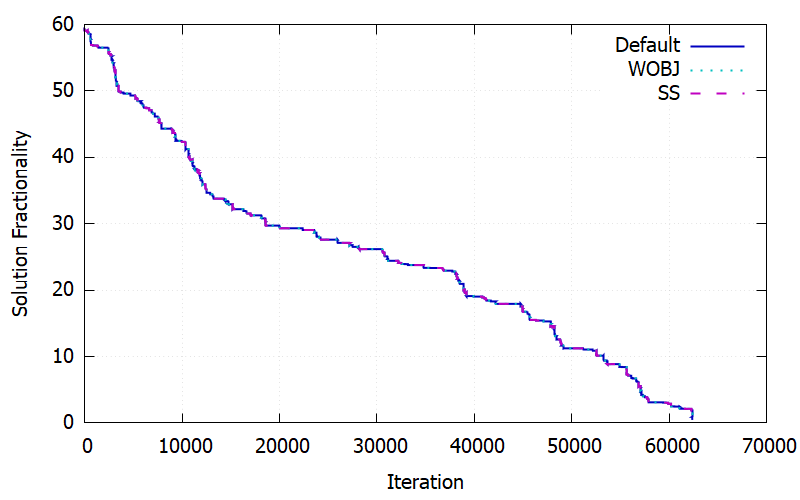
\includegraphics[width=0.85\textwidth]{fast0507-solfrac-worst.png}
	\caption{Solution fractionality of ZI-Round executions for the instance \texttt{fast0507}: worst-performing versions, in terms of number of iterations taken to round all the fractional integer variables.}
	\label{fig:fast0507-solfrac-worst}
\end{figure}

\begin{figure}[h!]
	\centering
	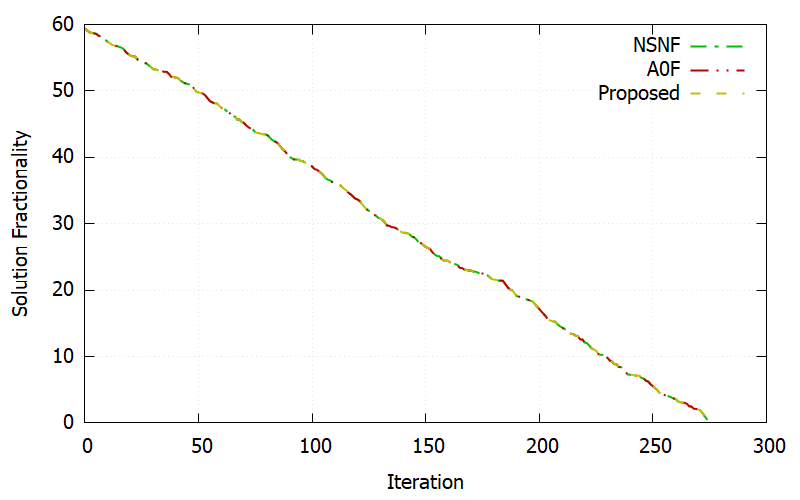
\includegraphics[width=0.85\textwidth]{fast0507-solfrac-best.png}
	\caption{Solution fractionality of ZI-Round executions for the instance \texttt{fast0507}: best-performing versions, in terms of number of iterations taken to round all the fractional integer variables.}
	\label{fig:fast0507-solfrac-best}
\end{figure}

All the three worst-performing versions present the two interfering phases of rounding and objective improvement, whereas all the three best-performing versions present a clear separation of the two phases, or the lack of one. The proposed version of ZI-Round clearly inherits the fast rounding phase from the extension that avoids improving the objective value while roundable fractional integer variables are still available. Notice the high delay in the rounding phase caused by the interference of the objective improvement phase for the instance \texttt{fast0507}: from $275$ iterations in Figure~\ref{fig:fast0507-solfrac-best} to more than $60000$ iterations in Figure~\ref{fig:fast0507-solfrac-worst}. \par
 
%! Solution fractionality seymour
For the instance \texttt{seymour}, the solution fractionality curves of all the ZI-Round versions tested are presented in a single chart in Figure~\ref{fig:seymour-solfrac-all}.

\begin{figure}[ht]
	\centering
	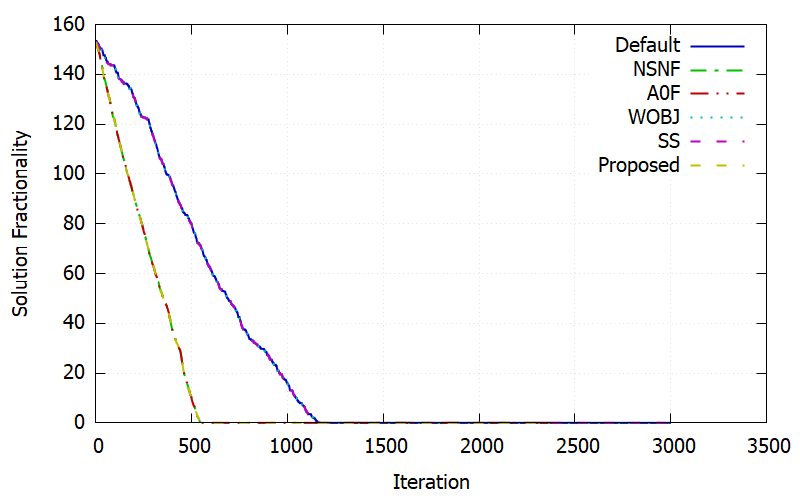
\includegraphics[width=0.85\textwidth]{seymour-solfrac-all.png}
	\caption{Solution fractionality of ZI-Round executions for the instance \texttt{seymour}: all versions.}
	\label{fig:seymour-solfrac-all}
\end{figure}

The same distinction of the worst-performing and best-performing versions made for the instance \texttt{fast0507} applies. In this case, though, the delay in the rounding phase caused by the interference of the objective improvement phase is less significative but still not negligible. As stated before, the proposed version of ZI-Round inherits the fast rounding phase from the extension that avoids improving the objective value while roundable fractional integer variables are stil available. \par

%! Solution cost fast0507
For the instance \texttt{fast0507}, the solution cost curves of all the ZI-Round versions tested are presented in a single chart in Figure~\ref{fig:fast0507-solcost-all}. The chart corresponding to the version that does not improve the objective value is also presented as a standalone chart in Figure~\ref{fig:fast0507-solcost-nsnf}, since it is not visible in the main chart, due to its high scale difference with respect to the charts of all the other versions.

\begin{figure}[ht]
	\centering
	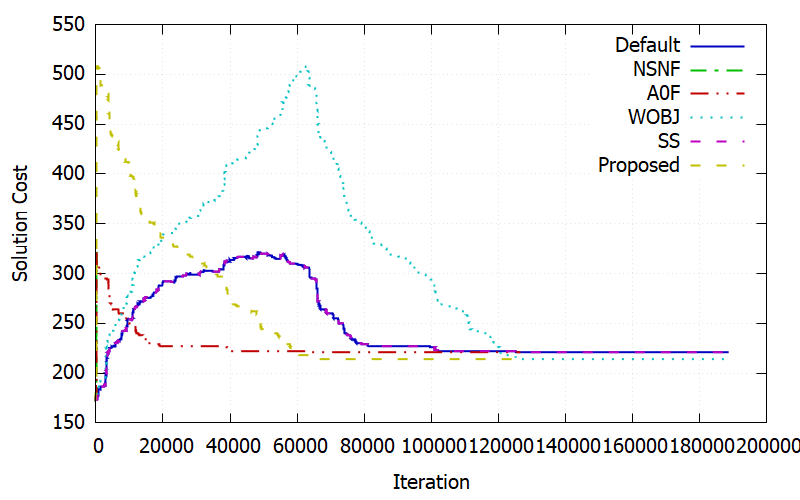
\includegraphics[width=0.85\textwidth]{fast0507-solcost-all.png}
	\caption{Solution cost of ZI-Round executions for the instance \texttt{fast0507}: all versions.}
	\label{fig:fast0507-solcost-all}
\end{figure}

\begin{figure}[h!]
	\centering
	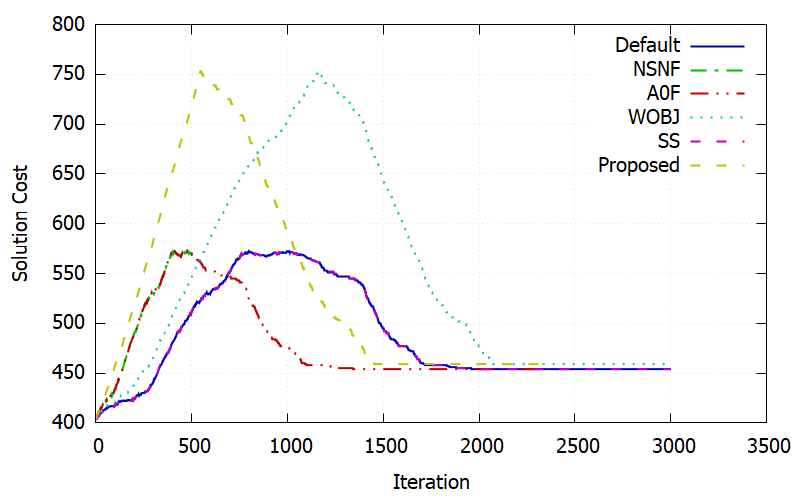
\includegraphics[width=0.85\textwidth]{seymour-solcost-all.png}
	\caption{Solution cost of ZI-Round executions for the instance \texttt{seymour}: all versions.}
	\label{fig:seymour-solcost-all}
\end{figure}

The three versions in which the two phases interfere with one another present a slow worsening of the objective value as the fractional integer variables are being rounded. When the solution fractionality finally reaches zero after more than $60000$ iterations, the objective improvement phase operates alone. 
The effect of rounding variables in the direction that worsens the objective value when fractionality tie-breaks occur is clearly visible in the solution cost curve of the corresponding version.
The two versions in which the two phases are separated, instead, present a fast worsening of the objective value, in terms of number of iterations. As soon as the fast rounding phase ends, the solution cost starts being improved. \par

%! Solution cost seymour
For the instance \texttt{seymour}, the solution cost curves of all the ZI-Round versions tested are presented in a single chart in Figure~\ref{fig:seymour-solcost-all}. The chart corresponding to the version that does not improve the objective value is also presented as a standalone chart in Figure~\ref{fig:seymour-solcost-nsnf}, since it is not visible in the main chart, due to its high scale difference with respect to the charts of all the other versions.

\begin{figure}[ht]
	\centering
	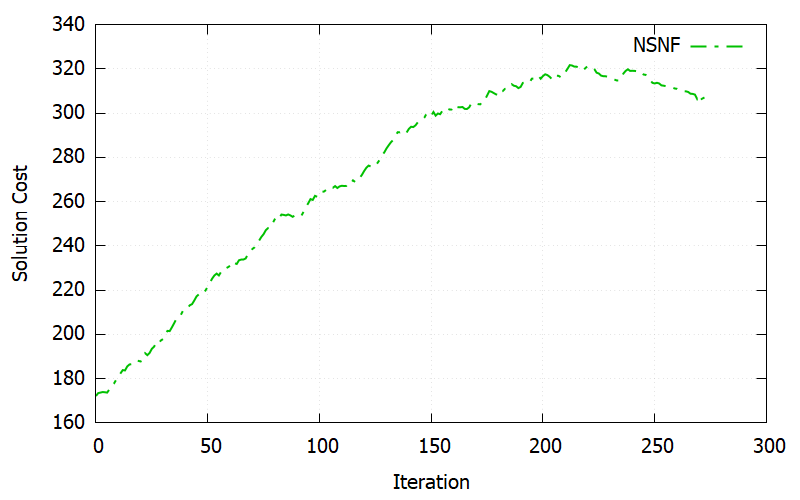
\includegraphics[width=0.83\textwidth]{fast0507-solcost-nsnf.png}
	\caption{Solution cost of ZI-Round execution for the instance \texttt{fast0507}: no objective improvement.}
	\label{fig:fast0507-solcost-nsnf}
\end{figure}

\begin{figure}[h!]
	\centering
	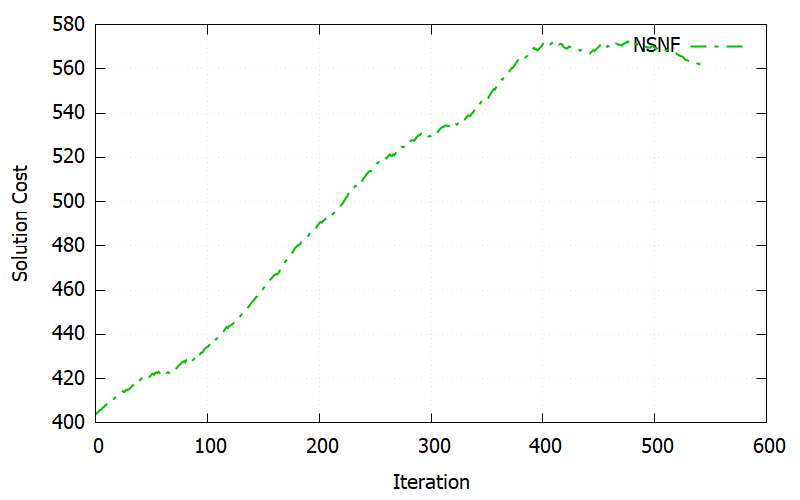
\includegraphics[width=0.83\textwidth]{seymour-solcost-nsnf.png}
	\caption{Solution cost of ZI-Round executions for the instance \texttt{seymour}: no objective improvement.}
	\label{fig:seymour-solcost-nsnf}
\end{figure}

The three versions in which the two phases interfere with one another present the same behavior observed for the instance \texttt{fast0507}, as well as the two versions in which the two phases are separated. \par 

The results obtained and the observations made allow to conclude that the proposed version of ZI-Round inherits its behaviors from the extension that penalizes the objective value when fractionality tie-breaks occur and the extension that keeps the two phases separated, specifically: the magnitude of the objective worsening from the former extension; the faster objective worsening from both extensions; the faster rounding phase from the latter extension.

%\begin{figure}[ht]
%	\centering
%	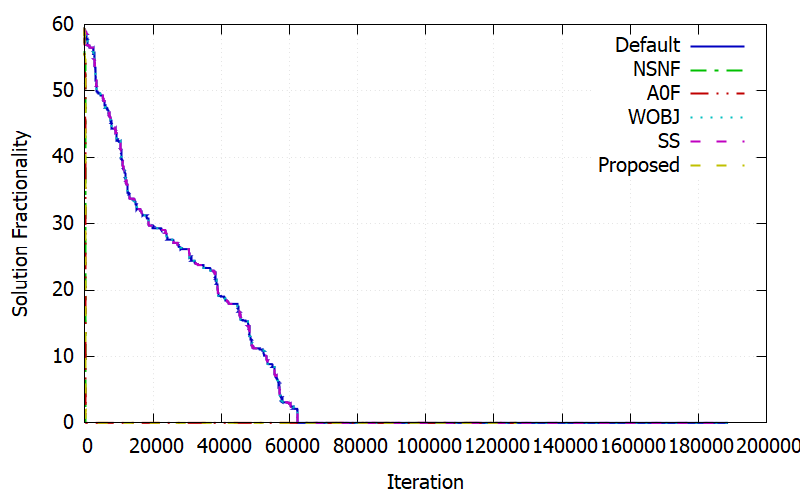
\includegraphics[width=0.85\textwidth]{fast0507-solfrac-all.png}
%	\caption{Solution fractionality of ZI-Round executions for the %instance \texttt{fast0507}: all versions.}
%	\label{fig:fast0507-solfrac-all}
%\end{figure}

%\begin{figure}[ht]
%	\centering
%	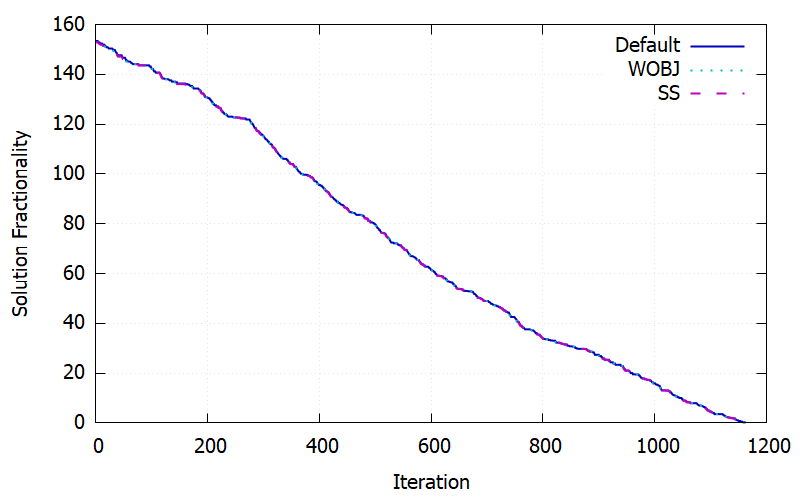
\includegraphics[width=0.85\textwidth]{seymour-solfrac-worst.png}
%	\caption{Solution fractionality of ZI-Round executions for the %instance \texttt{seymour}: worst versions.}
%	\label{fig:seymour-solfrac-worst}
%\end{figure}

%\begin{figure}[ht]
%	\centering
%	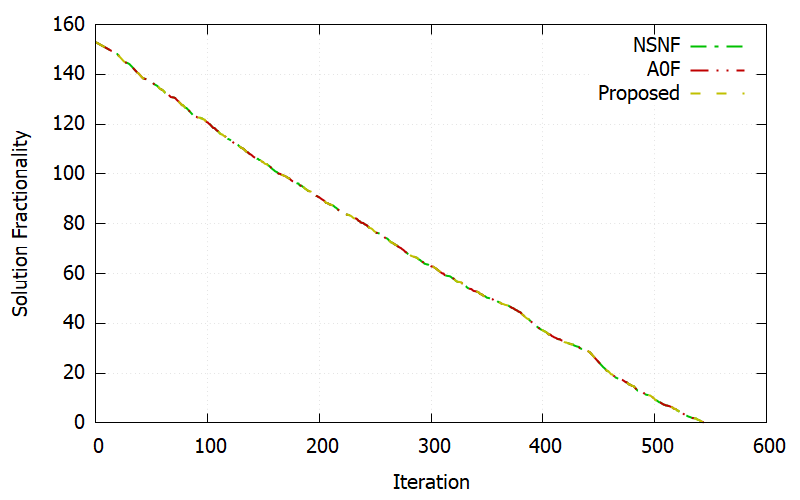
\includegraphics[width=0.85\textwidth]{seymour-solfrac-best.png}
%	\caption{Solution fractionality of ZI-Round executions for the %instance \texttt{seymour}: best versions.}
%	\label{fig:seymour-solfrac-best}
%\end{figure}

\renewcommand{\listfigurename}{Figures}
\listoffigures
\renewcommand{\listtablename}{Tables}
\listoftables

\nocite{*}
\renewcommand{\bibname}{References}
\begin{thebibliography}{9}
	
	\bibitem{wallace2010} C. Wallace, \textit{ZI round, a MIP rounding heuristic}. Journal of Heuristics, vol. 16, pp. 715–722 (2010). \\ DOI: \url{https://doi.org/10.1007/s10732-009-9114-6}

	\bibitem{linker1973} S. Lin, B. W. Kernighan, \textit{An Effective Heuristic Algorithm for the Traveling-Salesman Problem}. Operations Research, vol. 21, no. 2, pp. 498-516, INFORMS (1973). \\ DOI: \url{https://doi.org/10.1287/opre.21.2.498}

	\bibitem{christophel2005} P. M. Christophel, \textit{An Improved Heuristic for the MOPS Mixed-Integer Programming Solver}. University of Paderborn-DS\&OR Lab, Diplomarbeit (2005).

	\bibitem{berthold2006} T. Berthold, \textit{Primal Heuristics for Mixed Integer Programs}. Technische Universität Berlin, Diplomarbeit (2006).

	\bibitem{hendel2011} G. Hendel, \textit{New Rounding and Propagation Heuristics for Mixed Integer Programming}. Technische Universität Berlin, Bachelorarbeit (2011).

	\bibitem{achterberg2012} T. Achterberg, T. Berthold, G. Hendel, \textit{Rounding and Propagation Heuristics for Mixed Integer Programming}. In: D. Klatte, HJ. Lüthi, K. Schmedders (eds) "Operations Research Proceedings 2011". Operations Research Proceedings (GOR (Gesellschaft für Operations Research e.V.)). Springer, Berlin, Heidelberg (2012). \\ DOI: \url{https://doi.org/10.1007/978-3-642-29210-1_12}

	\bibitem{achterberg2013} T. Achterberg, R. Wunderling. \textit{Mixed Integer Programming: Analyzing 12 Years of Progress}. In: M. Jünger, G. Reinelt (eds) "Facets of Combinatorial Optimization". Springer, Berlin, Heidelberg (2013). \\ DOI: \url{https://doi.org/10.1007/978-3-642-38189-8_18}
	
	% \newpage
	\vspace{0.5cm}
	%* SITOGRAPHY %%%%%%%%%%%%%%%%%%%%%%%%%%%%%%%%%%%%%%%%%%%%%%%%%%%%%%%%%%%%
	\textsc{\Large \textbf{Sitography}}
	%*%%%%%%%%%%%%%%%%%%%%%%%%%%%%%%%%%%%%%%%%%%%%%%%%%%%%%%%%%%%%%%%%%%%%%%%%

	\bibitem{cplex} IBM ILOG CPLEX Optimization Studio. \\ URL: \url{https://www.ibm.com/products/ilog-cplex-optimization-studio} \\ (last visited: )

	\bibitem{scip} SCIP MIP solver (non-commercial). \\ URL: \url{https://www.scipopt.org/} \\ (last visited: )

	\bibitem{dirent} Dirent C API. \\ URL: \url{https://github.com/tronkko/dirent} \\ (last visited: )

	\bibitem{gnuplot} Gnuplot graphing utility. \\ URL: \url{http://www.gnuplot.info/} \\ (last visited: )

	\bibitem{rlang} R project. \\ URL: \url{https://www.r-project.org/} \\ (last visited: )

	\bibitem{miplib2003} MIPLIB 2003. \\ URL: \url{http://miplib2010.zib.de/miplib2003/} \\ (last visited: )

	\bibitem{miplib2010} MIPLIB 2010. \\ URL: \url{http://miplib2010.zib.de/} \\ (last visited: )

	\bibitem{miplib2017} MIPLIB 2017. \\ URL: \url{http://miplib.zib.de/} \\ (last visited: )
	
\end{thebibliography}

\end{document}